\documentclass{snedecorbeamer}

\addtobeamertemplate{footnote}{\hskip -4ex}{}

\usepackage{natbib}

\graphicspath{{inc/}}
\usetikzlibrary{positioning,decorations.pathreplacing,quotes,overlay-beamer-styles}

\hypersetup{
  colorlinks,
  citecolor=violet,
  linkcolor=orange,
  urlcolor=blue
}

\usepackage{tcolorbox}
\newenvironment{infoblock}
{ \begin{tcolorbox}[colback=green!5!white,colframe=green!75!black] }
  { \end{tcolorbox} }

\begin{document}

% Title page -------------------------------------------------------------------
\title{Automatic Dynamic Relevance Determination}
\subtitle{A methodology for Gaussian process regression\\
  with high-dimensional functional inputs}
\date{October 10, 2022}

\institute{
  \inst{1}Department of Statistics, Iowa State University \\
  \inst{2}NASA Jet Propulsion Laboratory \\
  \inst{3}Departments of Statistics, and IMSE, Iowa State University
}

\renewcommand*{\thefootnote}{\fnsymbol{footnote}}
\author{
  \textbf{Luis Damiano}\footnote[2]{
    \tiny{\href{mailto:ldamiano@iastate.edu}{ldamiano@iastate.edu}}%
    \newline
    \tiny{Submitted to Technometrics:
      \href{https://doi.org/10.48550/arXiv.2209.00044}{10.48550/arXiv.2209.00044}}
  }\inst{1},
  Margaret Johnson\inst{2},
  Joaquim Teixeira\inst{2},
  Max D. Morris\inst{3},
  Jarad Niemi\inst{1}}

\begin{frame}
  \titlepage{}
\end{frame}

% Intro ------------------------------------------------------------------------
\begin{frame}
  \frametitle{Case study}
  \framesubtitle{NASA's Microwave Limb Sounder}

  \begin{columns}[t]
    \begin{column}{.50\textwidth}
      \begin{center}
        \vspace{-2ex}

        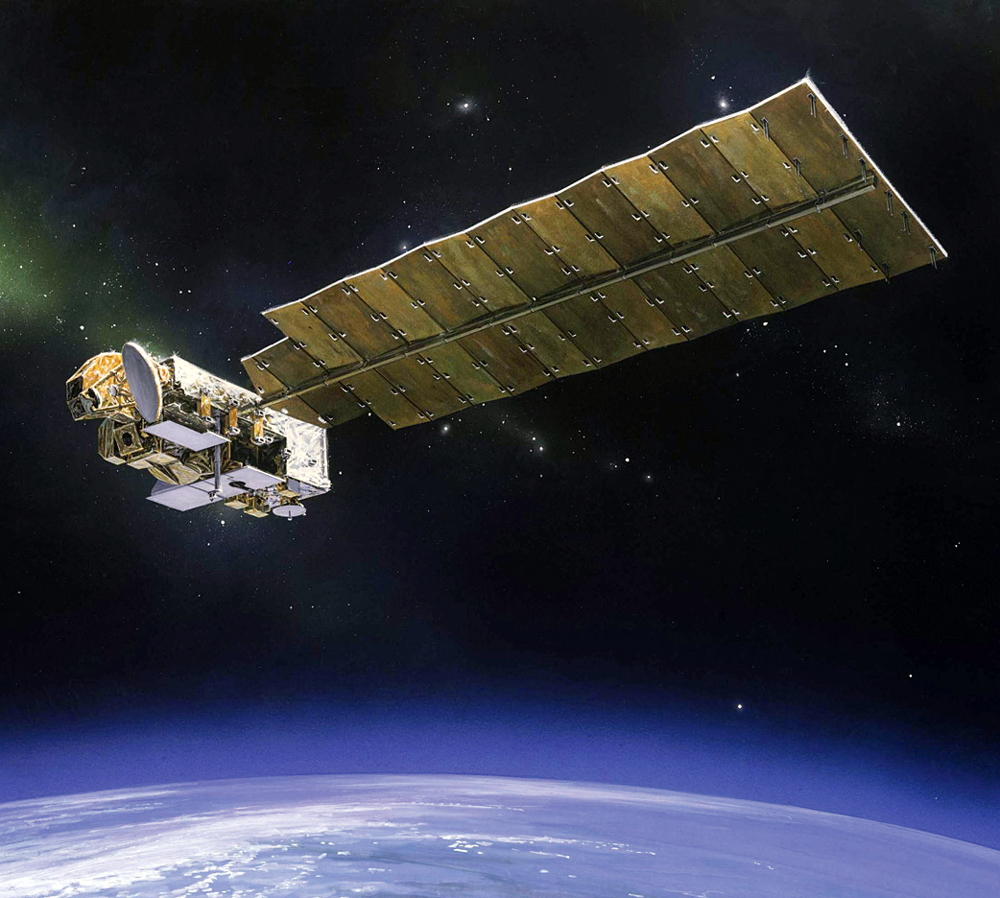
\includegraphics[height=.4\textheight]{aura.jpg}

        {\footnotesize \textit{Credit: NASA Aura}}

        \vspace{5ex}

        \definecolor{bright-spark}{RGB}{255, 195, 59}
        \tikzstyle{nice-rectangle} = [rectangle, rounded corners,
        minimum width=3cm, minimum height=1cm, text centered,
        fill=bright-spark, font=\sffamily]
        \tikzset{every label/.style={font=\itshape\footnotesize}}%
        \begin{adjustbox}{width=.66\textwidth}
        \begin{tikzpicture}
          \node (input) [nice-rectangle] [text width = 15ex] [label=below:Functional
          input $X(t)$] {Atmospheric constituents};
          \node
          (output) [nice-rectangle, right=of input]
          [label=below:Scalar output $y$] {Radiance};
          \draw [->] (input) [above] -- node {$f$} (output);
        \end{tikzpicture}
        \end{adjustbox}
      \end{center}
    \end{column}
    \begin{column}{.50\textwidth}
      \begin{tikzpicture}[overlay, remember picture]
        \node[anchor=north west] (b) at (-.2, .9) {
          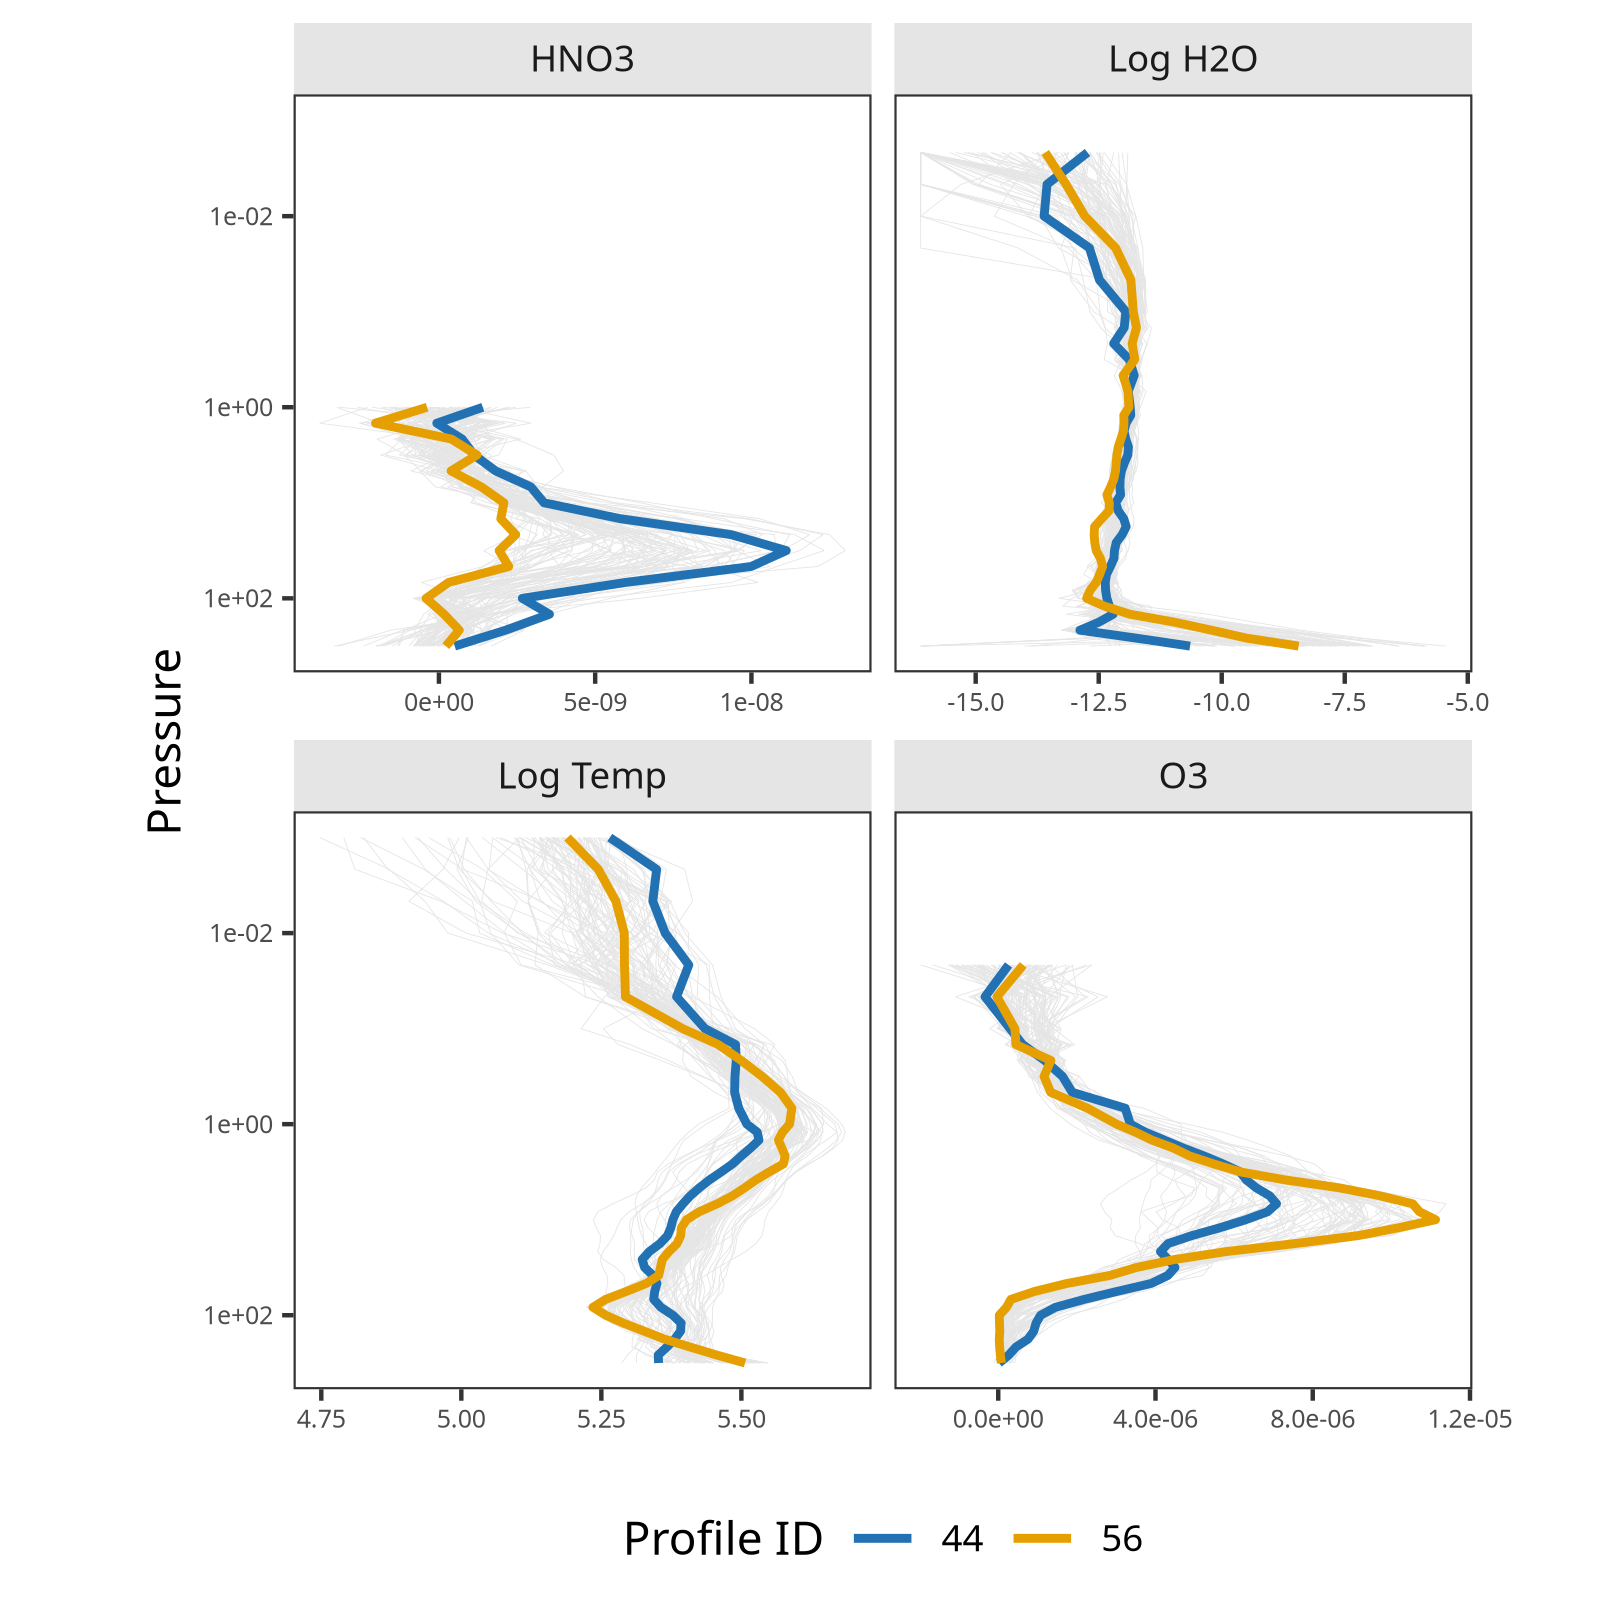
\includegraphics[height=.9\textheight]{14-exploratory-profiles-vertical.png}
        };
      \end{tikzpicture}
    \end{column}
  \end{columns}
\end{frame}

% Methods ----------------------------------------------------------------------
\begin{frame}
  \frametitle{Functional Input Gaussian Process (fiGP)}
  \framesubtitle{From ARD to ADRD}

  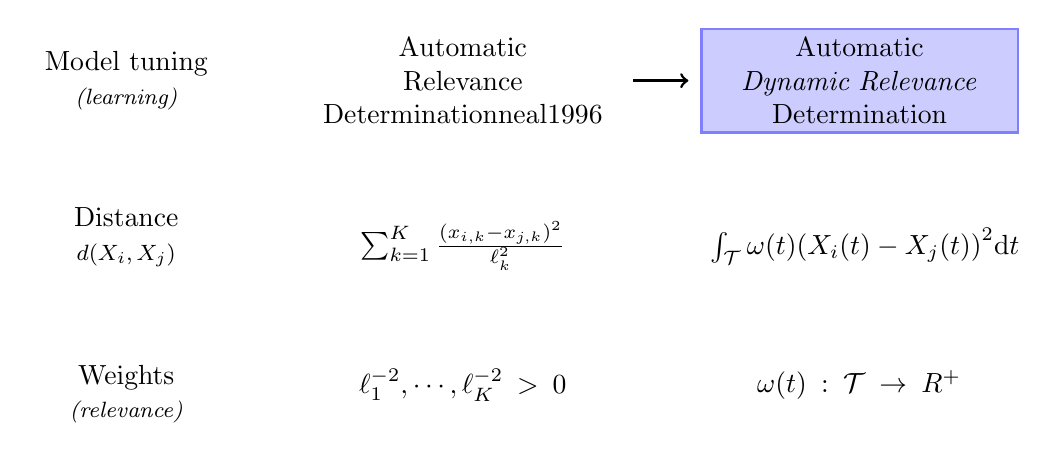
\begin{tikzpicture}
    [
    txtbox1/.style={rectangle,align=center,draw=blue!50,fill=blue!20,thick},
    every label/.style={font=\itshape\footnotesize}
    ]
    \tikzset{every node/.style={align=center}}
    \node (aspect1b)   at (0, 0)                        [text width=15ex] {
      Model tuning\\{\footnotesize \itshape (learning)}
    };
    \node (aspect2)    [below=of aspect1b]              [text width=15ex] {
      Distance\\{\footnotesize $d(X_i, X_j)$}
    };
    \node (aspect3)    [below=of aspect2]               [text width=15ex] {
      Weights\\{\footnotesize \itshape (relevance)}
    };
    %%%%%
    \node (solution1b) [right=of aspect1b]              [text width=25ex] {
      Automatic\\Relevance\\Determination\citep{neal1996}
    };
    %%%%%
    \node (solution2b) [txtbox1] [right=of solution1b]  [text
    width=25ex]
    [visible on=<2->]{
      Automatic\\\textit{Dynamic Relevance}\\Determination
    };
    %%%%%
    \node (eq1b) [below=of solution1b] [text width=25ex] {
      $\sum_{k=1}^K \frac{{(x_{i, k} - x_{j, k})}^2}{\ell_k^2}$
    };
    % \node (eq2b) [below=of solution2b] [text width=25ex]
    \node (eq2b) [right=of eq1b] [text width=25ex]
    [visible on=<2->]{
      $\int_{\mathcal{T}}
      \omega(t)
      {\left(X_i(t) - X_j(t) \right)}^2 \mathrm{d}t
      $
    };
    %%%%%
    \node (par1b) [below=of eq1b] [text width=25ex]{
      $\ell^{-2}_1, \cdots, \ell^{-2}_K > 0$
    };
    % \node (par2b) [below=of eq2b] [text width=25ex]
    \node (par2b) [right=of par1b] [text width=25ex]
    [visible on=<2->]{
      $\omega(t): \mathcal{T} \to \mathbb{R}^+$
    };
    \draw[shorten >=1ex,shorten <=1ex,line width=1pt]
    [visible on=<2->] [->] (solution1b.east) -- (solution2b.west);
    % \draw[shorten >=1ex,shorten <=1ex,line width=1pt]
    % [visible on=<3->] [->] (eq1b.east) -- (eq2b.west);
    % \draw[shorten >=1ex,shorten <=1ex,line width=1pt]
    % [visible on=<4->] [->] (par1b.east) -- (par2b.west);
  \end{tikzpicture}
  \begin{infoblock}
    Risk of overfitting as $K\to\infty$
  \end{infoblock}
\end{frame}

\begin{frame}
  \frametitle{Functional Input Gaussian Process (fiGP)}
  \framesubtitle{Automatic Dynamic Relevance Determination}

  \begin{align}
    \mathbf{y}
    &\sim \mathcal{N}\left(0, \sigma_{f}^{2} \ \mathbf{R}_f
      + \sigma_{\varepsilon}^{2}\mathbf{I}\right) \\
    {\left(\mathbf{R}_f\right)}_{ij}
    &=
      \text{exp}\left\{
      -0.5 \phi^{-2} \ d_f(X_i, X_j)
      \right\} \\
    \visible<1->{
    d_f(X_i, X_j)
    &= \int_{\mathcal{T}}
      \omega(t)
      {\left(X_i(t) - X_j(t) \right)}^2 dt
      } \\
    \visible<1->{
    \omega(t)
    &: \mathcal{T}\to\mathbb{R}^+
      }
  \end{align}

  \blankfootnote{
    $\sigma_{\varepsilon}^2 > 0$,
    $\sigma_{f}^2 > 0$,
    $\phi > 0$,
    $i, j = 1, \dots, N, N\in\mathbb{N}$
  }
\end{frame}

\begin{frame}
  \frametitle{Asymmetrical Laplace function}
  \framesubtitle{Specification}

  \begin{figure}[h!]
	\centering
    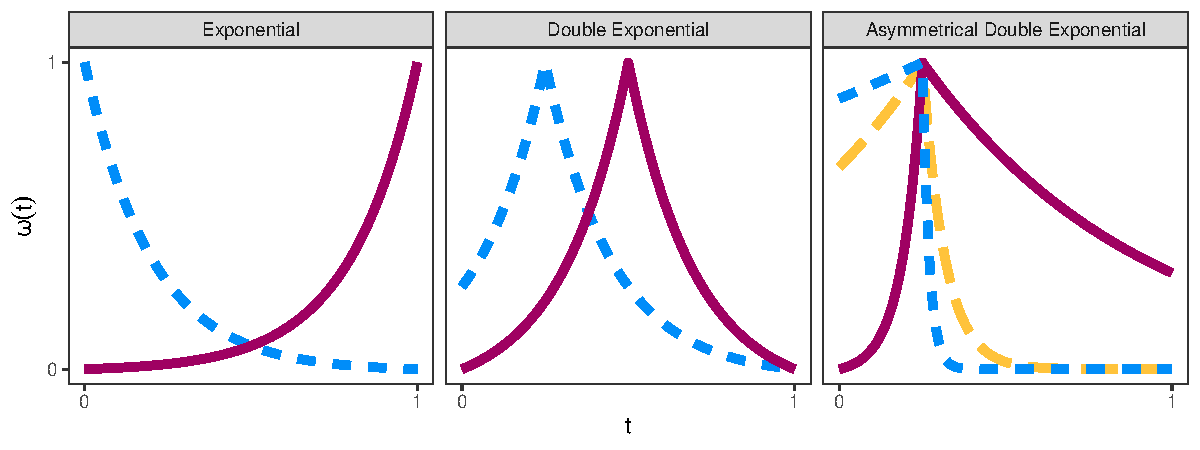
\includegraphics[width=.7\textwidth]{02-alf-weight-plot}%
  \end{figure}
  \vspace{-8ex}
  \begin{center}
    \begin{align}
      \omega(t)
      &= \text{exp}\left\{-(t - \tau) \lambda \kappa^s s\right\} \\
      &= {
        \tiny
        \begin{cases}
          \text{exp}\left(- \lambda_1 \ \lvert t - \tau \rvert
          \right) & \text{for } t \le \tau \\
          \text{exp}\left(- \lambda_2 \ \lvert t - \tau \rvert
          \right) & \text{for } t > \tau \\
        \end{cases}
      }\nonumber
    \end{align}
  \end{center}

  \blankfootnote{
    $\omega(t): \mathcal{T} = [0, 1] \to (0, 1]$,
    $s = \text{sign}(t - \tau)$,
    $\tau \in[0, 1]$,
    $\lambda > 0$,
    $\kappa > 0$
    \newline
    Priors:
    $\tau \sim \textsc{Beta}$,
    $\lambda \sim \textsc{N}^{+}$,
    $\log(\kappa) \sim \textsc{N}$
  }
\end{frame}

% Case study -------------------------------------------------------------------
\begin{frame}
  \frametitle{Case study}
  \framesubtitle{Implementation}

  \begin{itemize}
  \item 8 training and 8 test complementary sets with 1,000 soundings each
  \item 7 plausible models
    \begin{itemize}
    \item viGP SE, ARD, FPCA, FFPCA
    \item fiGP Edn, SDE, ADE
    \item One model fit separately per input-output pair
    \end{itemize}
  \item Fully Bayesian inference
    \begin{itemize}
    \item Hamiltonian Monte Carlo~\citep[ch. 5]{brooks2011}
    \item NUTS algorithm~\citep{hoffman2014} via Stan~\citep{standevelopmentteam2021}
    \item 1 long chain~\citep{raftery1992}
    \item Extensive search for an initial value
    \item 500 post-warmup iterations
    \item 1,500 posterior samples
    \end{itemize}
  \item Several out-of-sample validation statistics
    \hyperlink{frm:validation}{\beamerbutton{see more}}
  \end{itemize}
\end{frame}

\begin{frame}[c]
  \begin{figure}
    \centering
    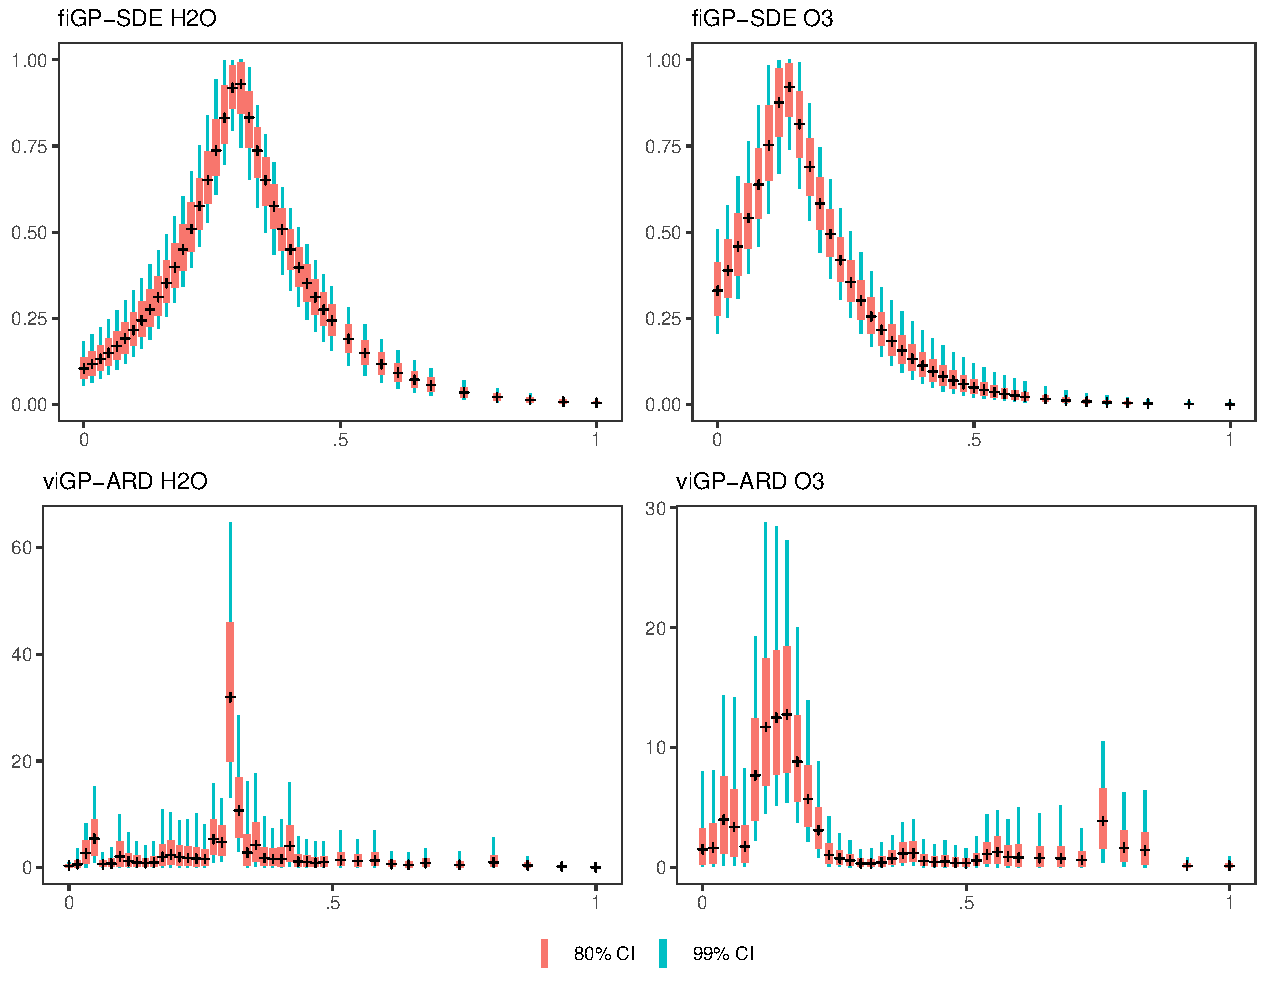
\includegraphics[height=.95\textheight]{weights-examples-pressure.pdf}
  \end{figure}

  \blankfootnote{In this slide only, we fix $\kappa = 1$ so that
    $\omega(t)$ is symmetrical}
\end{frame}

\begin{frame}[c]
  \begin{figure}
    \centering
    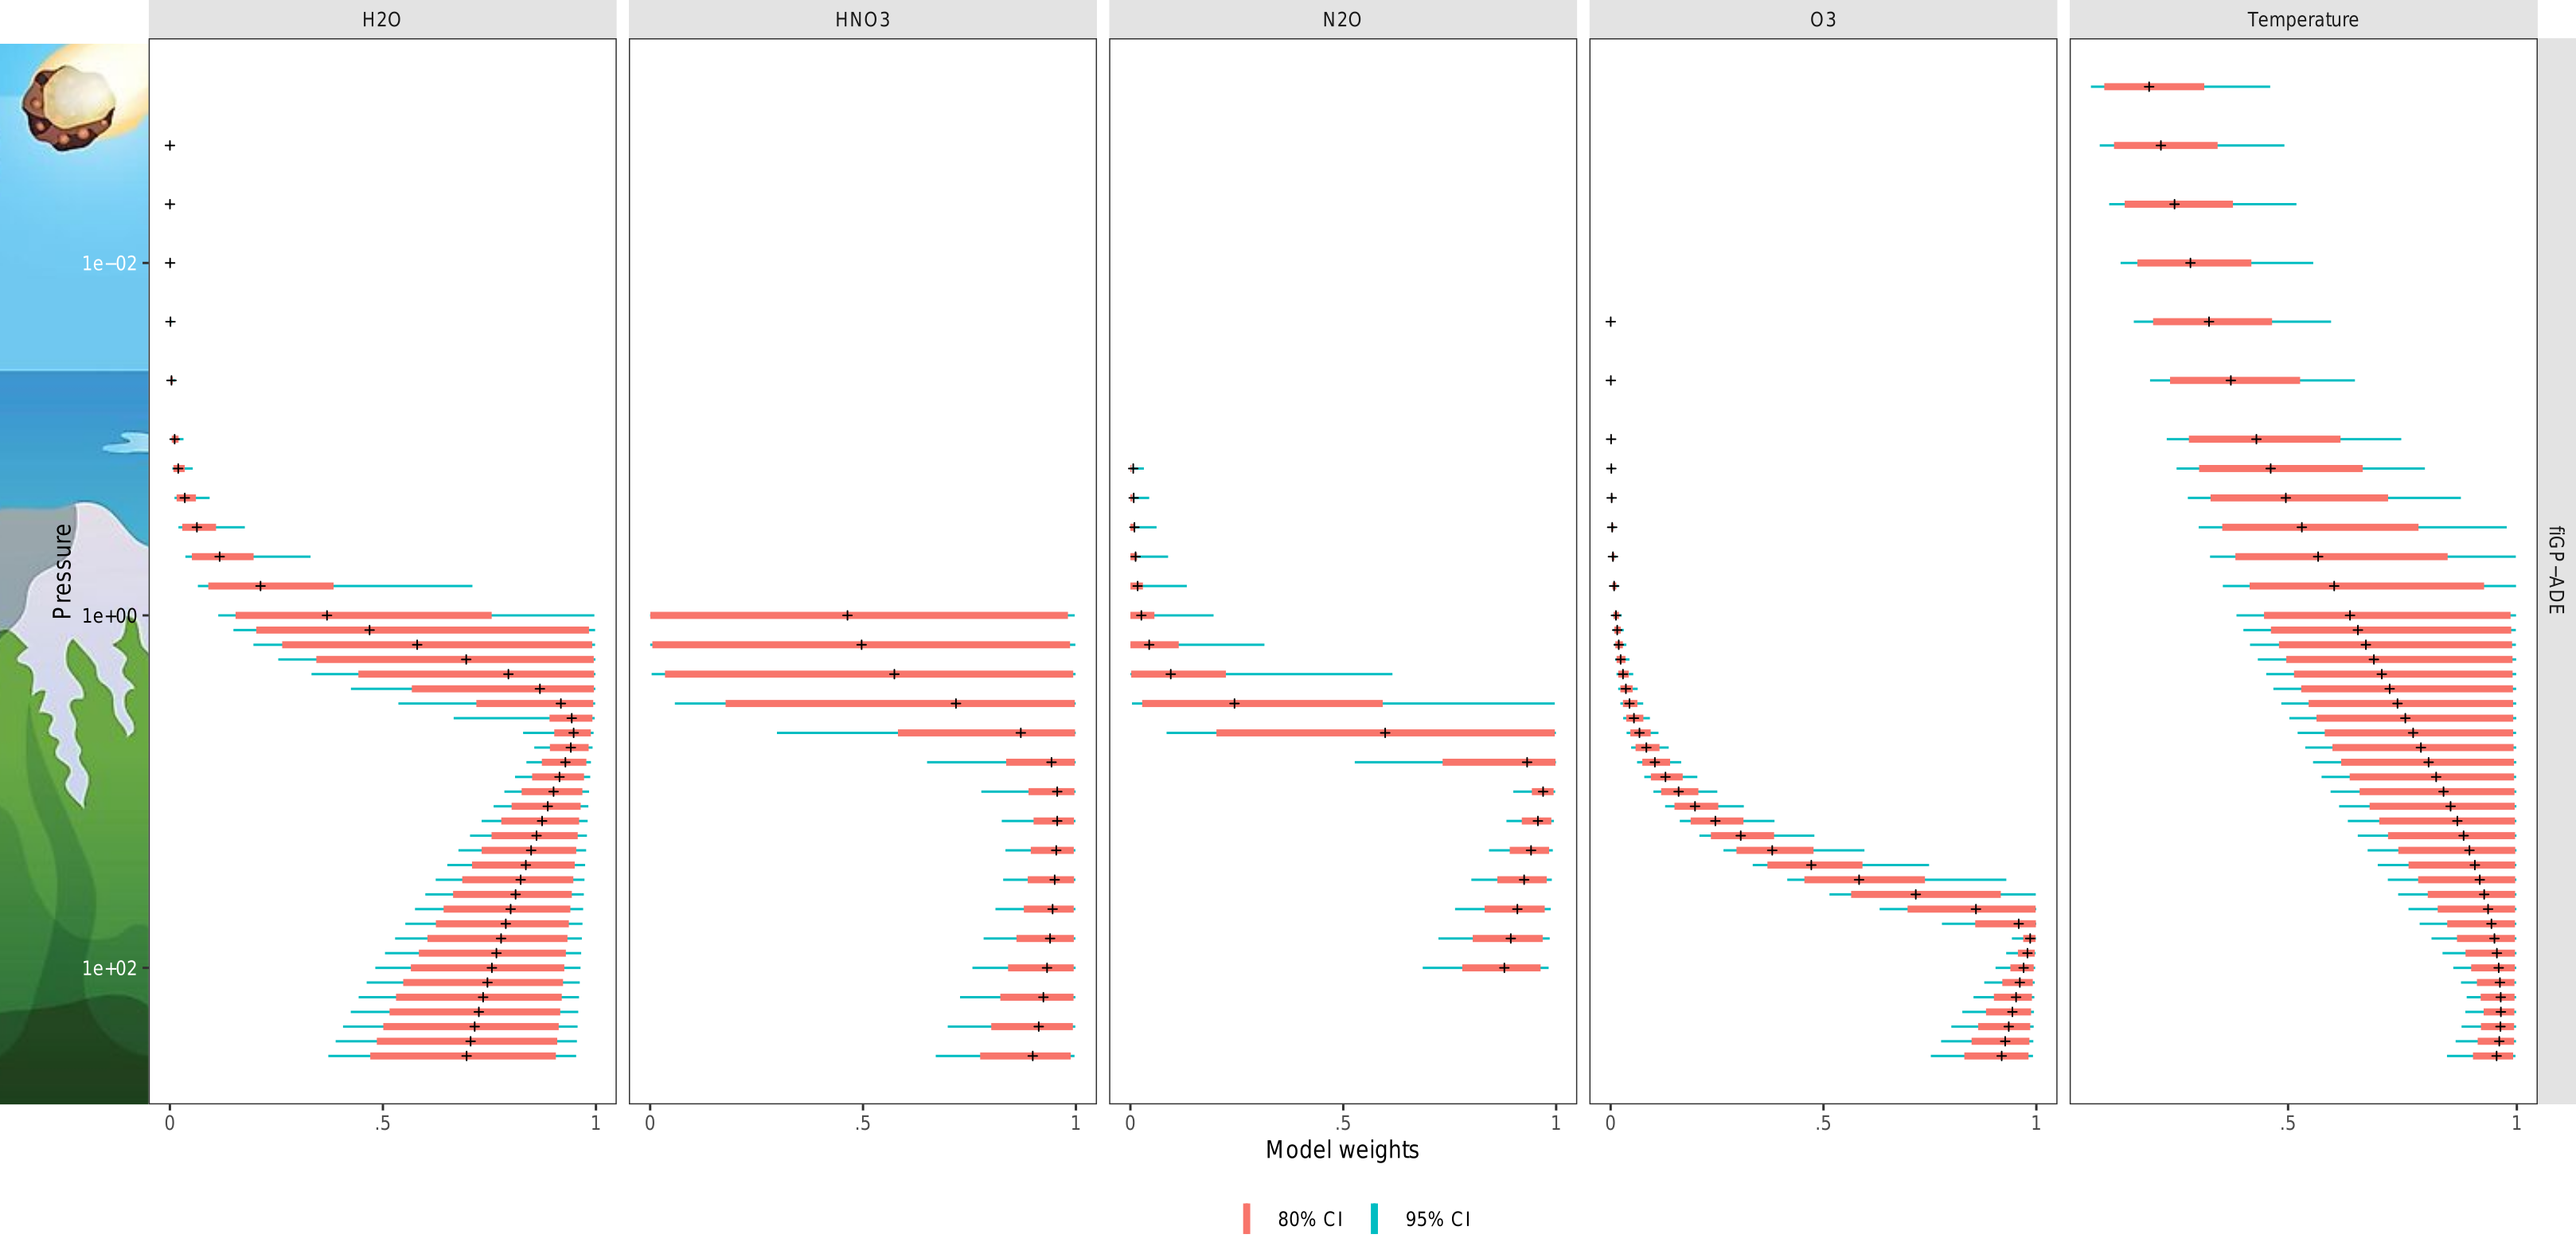
\includegraphics[width=1\textwidth]{image2934-8.png}
  \end{figure}
\end{frame}

\begin{frame}
  \frametitle{In summary}

  \begingroup
  \setbeamersize{description width=-\labelsep}
  \begin{description}[<+->]
  \item[No dimension reduction] \mbox{}\\
    better prediction than \textsc{FPCA}
  \item[Parsimony] \mbox{}\\
    competitive prediction with fewer parameters than \textsc{ARD}
  \item[Interpretability] \mbox{}\\
    $\omega(t) | \mathbf{y}$ may provide information about the underlying
    physical process
  \item[Smoothness] \mbox{}\\
    in relevance over the vertical grid to penalize noisy patterns
  \item[Next steps] \mbox{}\\
    explore multimodality in the relevance pattern
  \end{description}
  \endgroup
\end{frame}

% Closing slide ----------------------------------------------------------------
\begin{frame}[c]
  \frametitle{Acknowledgments}
  \centering

  {\small Jarad Niemi (ISU), Max D. Morris (ISU)\\
    Margaret Johnson (JPL), Joaquim Texeira (JPL) \\
    Microwave Limb Sounder team (JPL)\\
    ISU PIRI on C-CHANGE:~Science for a Changing Agriculture\\
    Foundation for Food and Agriculture Research}

  \vfill

  {\huge Thank you!}

  \vfill

  {\tiny References and extra slides on the back}

  \href{ldamiano@iastate.edu}{\beamergotobutton{mail}
    ldamiano@iastate.edu}

  \href{https://luisdamiano.github.io/}{\beamergotobutton{site}
    luisdamiano.github.io}

  \vfill

\end{frame}

% Appendix ---------------------------------------------------------------------
\appendix

\section{References}

\setbeamertemplate{bibliography item}{\insertbiblabel}

\begin{frame}[allowframebreaks]{References}
  \tiny
  \bibliographystyle{unsrt}
  \bibliography{references}
\end{frame}

\begin{frame}
  \frametitle{Literature review}
  \framesubtitle{}

  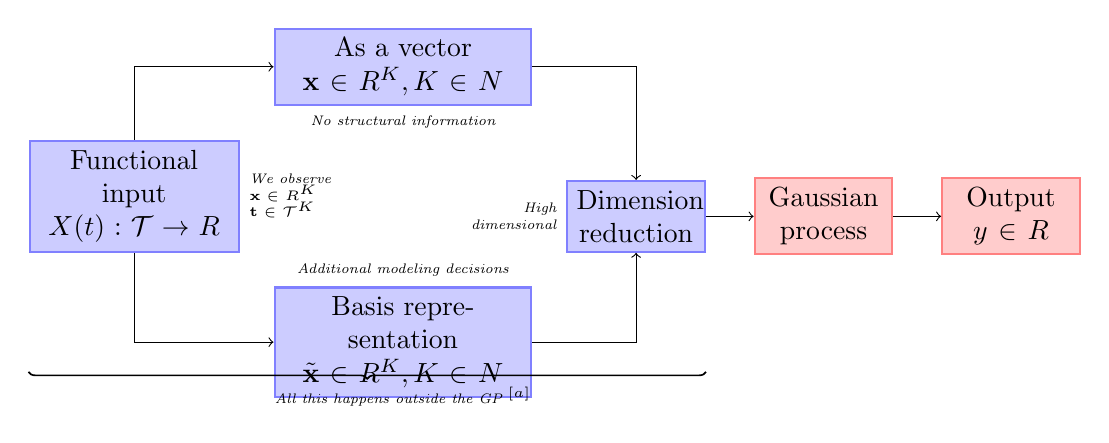
\begin{tikzpicture}
    [
    txtbox1/.style={rectangle,align=center,draw=blue!50,fill=blue!20,thick},
    txtbox2/.style={rectangle,align=center,draw=red!50,fill=red!20,thick},
    every label/.style={font=\itshape\tiny}
    ]

    \node (inp)  [txtbox1] at ( 0,  0) [text width=16ex]
    [label={[align=left]right:We observe \\ $\mathbf{x} \in \mathbb{R}^K$\\ $\mathbf{t}\in\mathcal{T}^K$}] {
      Functional input \\
      $X(t): \mathcal{T} \to \mathbb{R}$
    };
    \visible<1->{
      \node (vec1) [txtbox1] [above right=4ex of inp]   [text width=20ex]
      [label=below:No structural information]{
        As a vector \\
        $\mathbf{x} \in \mathbb{R}^K, K \in \mathbb{N}$
      };
      \node (vec2) [txtbox1] [below right=4ex of inp]   [text width=20ex]
      [label=above:Additional modeling decisions]{
        Basis representation \\
        $\tilde{\mathbf{x}} \in \mathbb{R}^K, K \in \mathbb{N}$
      };
    }
    \visible<1->{
      \node (dred) [txtbox1] [above right=4ex of vec2] [text width=10ex]
      [label={[align=right]left:High\\dimensional}]
      {
        Dimension \\ reduction
      };
    }

    \node (gp)   [txtbox2] [right=4ex of dred] [text width=10ex] {
      Gaussian \\ process
    };
    \node (out)  [txtbox2] [right=4ex of gp] [text width=10ex]  {
      Output \\ $y \in \mathbb{R}$
    };
    \visible<1->{
      \node [below=6ex of vec2.north, label=below:All this happens outside the GP$~^{[a]}$] {
      };
    }
    \draw [->] [visible on=<1->] (inp.north) |- (vec1.west);
    \draw [->] [visible on=<1->] (inp.south) |- (vec2.west);
    \draw [->] [visible on=<1->] (vec1.east) -| (dred.north);
    \draw [->] [visible on=<1->] (vec2.east) -| (dred.south);
    \draw [->] [visible on=<1->] (dred.east) -- (gp.west);
    \draw [->] (gp.east)   -- (out.west);
    \path [visible on=<1->] (inp.south west)
    edge[decorate,decoration={brace,mirror,raise=10ex},line width=.6pt]
    (inp.south west -| dred.south east);
  \end{tikzpicture}

  {\footnotesize
    \begin{itemize}
    \item<1-> Can we connect the functional input structure to a physical
      mechanism?
    \item<1-> Can we incorporate the functional input structure into the GP?$~^{[b]}$
    \item<1-> Can we circumvent input dimension reduction?
    \end{itemize}
  }

  \blankfootnote{\visible<1->{
      $~^{[a]}$\cite{muehlenstaedt2017,nanty2016,wang2017,tan2019,wang2019,betancourt2020,betancourt2020a,li2021} \,
      $~^{[b]}$\cite{morris2012,kuttubekova2019}
    }}
\end{frame}

\begin{frame}%
  \label{frm:validation}
  \frametitle{Functional input Gaussian processes}
  \framesubtitle{Validation statistics}

  \newcommand{\predmean}{\hat{\mathbf{m}}^{y}_*}
  \newcommand{\predvar}{\hat{\mathbf{S}}^{y}_*}
  \newcommand{\postpred}{\hat{p}^{y}_*}

  \begin{itemize}
  \item   Let
    $\hat{\mathbf{m}} = \predmean = \{\hat{m}_{*n}: n = 1, \dots, N\} =
    \EV{\mathbf{y}_* | \mathbf{y}, \mathbf{X}, \mathbf{X}_*}$
    and
    $\hat{\mathbf{S}} = \predvar = \VV{\mathbf{y}_* |
      \mathbf{y}, \mathbf{X}, \mathbf{X}_*}$
    be the predictive mean vector and covariance matrix.
  \item  Define the
    prediction error vector $\mathbf{e} = \mathbf{e}_{*}^{y} =
    \mathbf{y}_{*} - \hat{\mathbf{m}}$.
  \item Define the square Mahalanobis distance $D^2
    = \mathbf{e}^{\transp} \hat{\mathbf{S}}^{-1} \mathbf{e}$.
  \item Define the point-wise 95\% coverage indicator variable
    $I_{n} = 1$ if $y_{*n} \in \hat{m}_{*n} \pm 1.96
    {\hat{S}_{nn}}^{-\frac{1}{2}}$.
  \item   Let $\bar{y}_* = N^{-1} \sum_{n=1}^{N} y_{*n}$ be the test output
    mean.
  \end{itemize}

  \begin{center}
    \begin{tabular}{lrl}
      RMSE
      & $v_{\textsc{RMSE}}$ =
      & $N^{-\frac{1}{2}} \norm{\mathbf{e}}$ \\
      $R^2$
      & $v_{\textsc{R2}} $ =
      & $1 -%
        \norm{\mathbf{e}}^{2}
        \norm{\mathbf{y}_* - \bar{y}_*}^{-2}$ \\
      PPLD
      & $v_{\textsc{PPLD}}$ =
      & $
        -\frac{1}{2} \log \lvert \hat{\mathbf{S}} \rvert
        -D^2
        -\frac{n}{2} \log 2 \pi
        $
      \\
      CRPS
      & $v_{\textsc{CRPS}}$ =
      & $
        -\log \lvert \hat{\mathbf{S}} \rvert%
        -D^2
        $
      \\
      Nominal coverage
      & $v_{\textsc{COV95}}$ =
      & $N^{-1} \sum_{n = 1}^{N} I_{n}$
    \end{tabular}
  \end{center}
\end{frame}

\begin{frame}[c]
  \begin{figure}
    \centering
    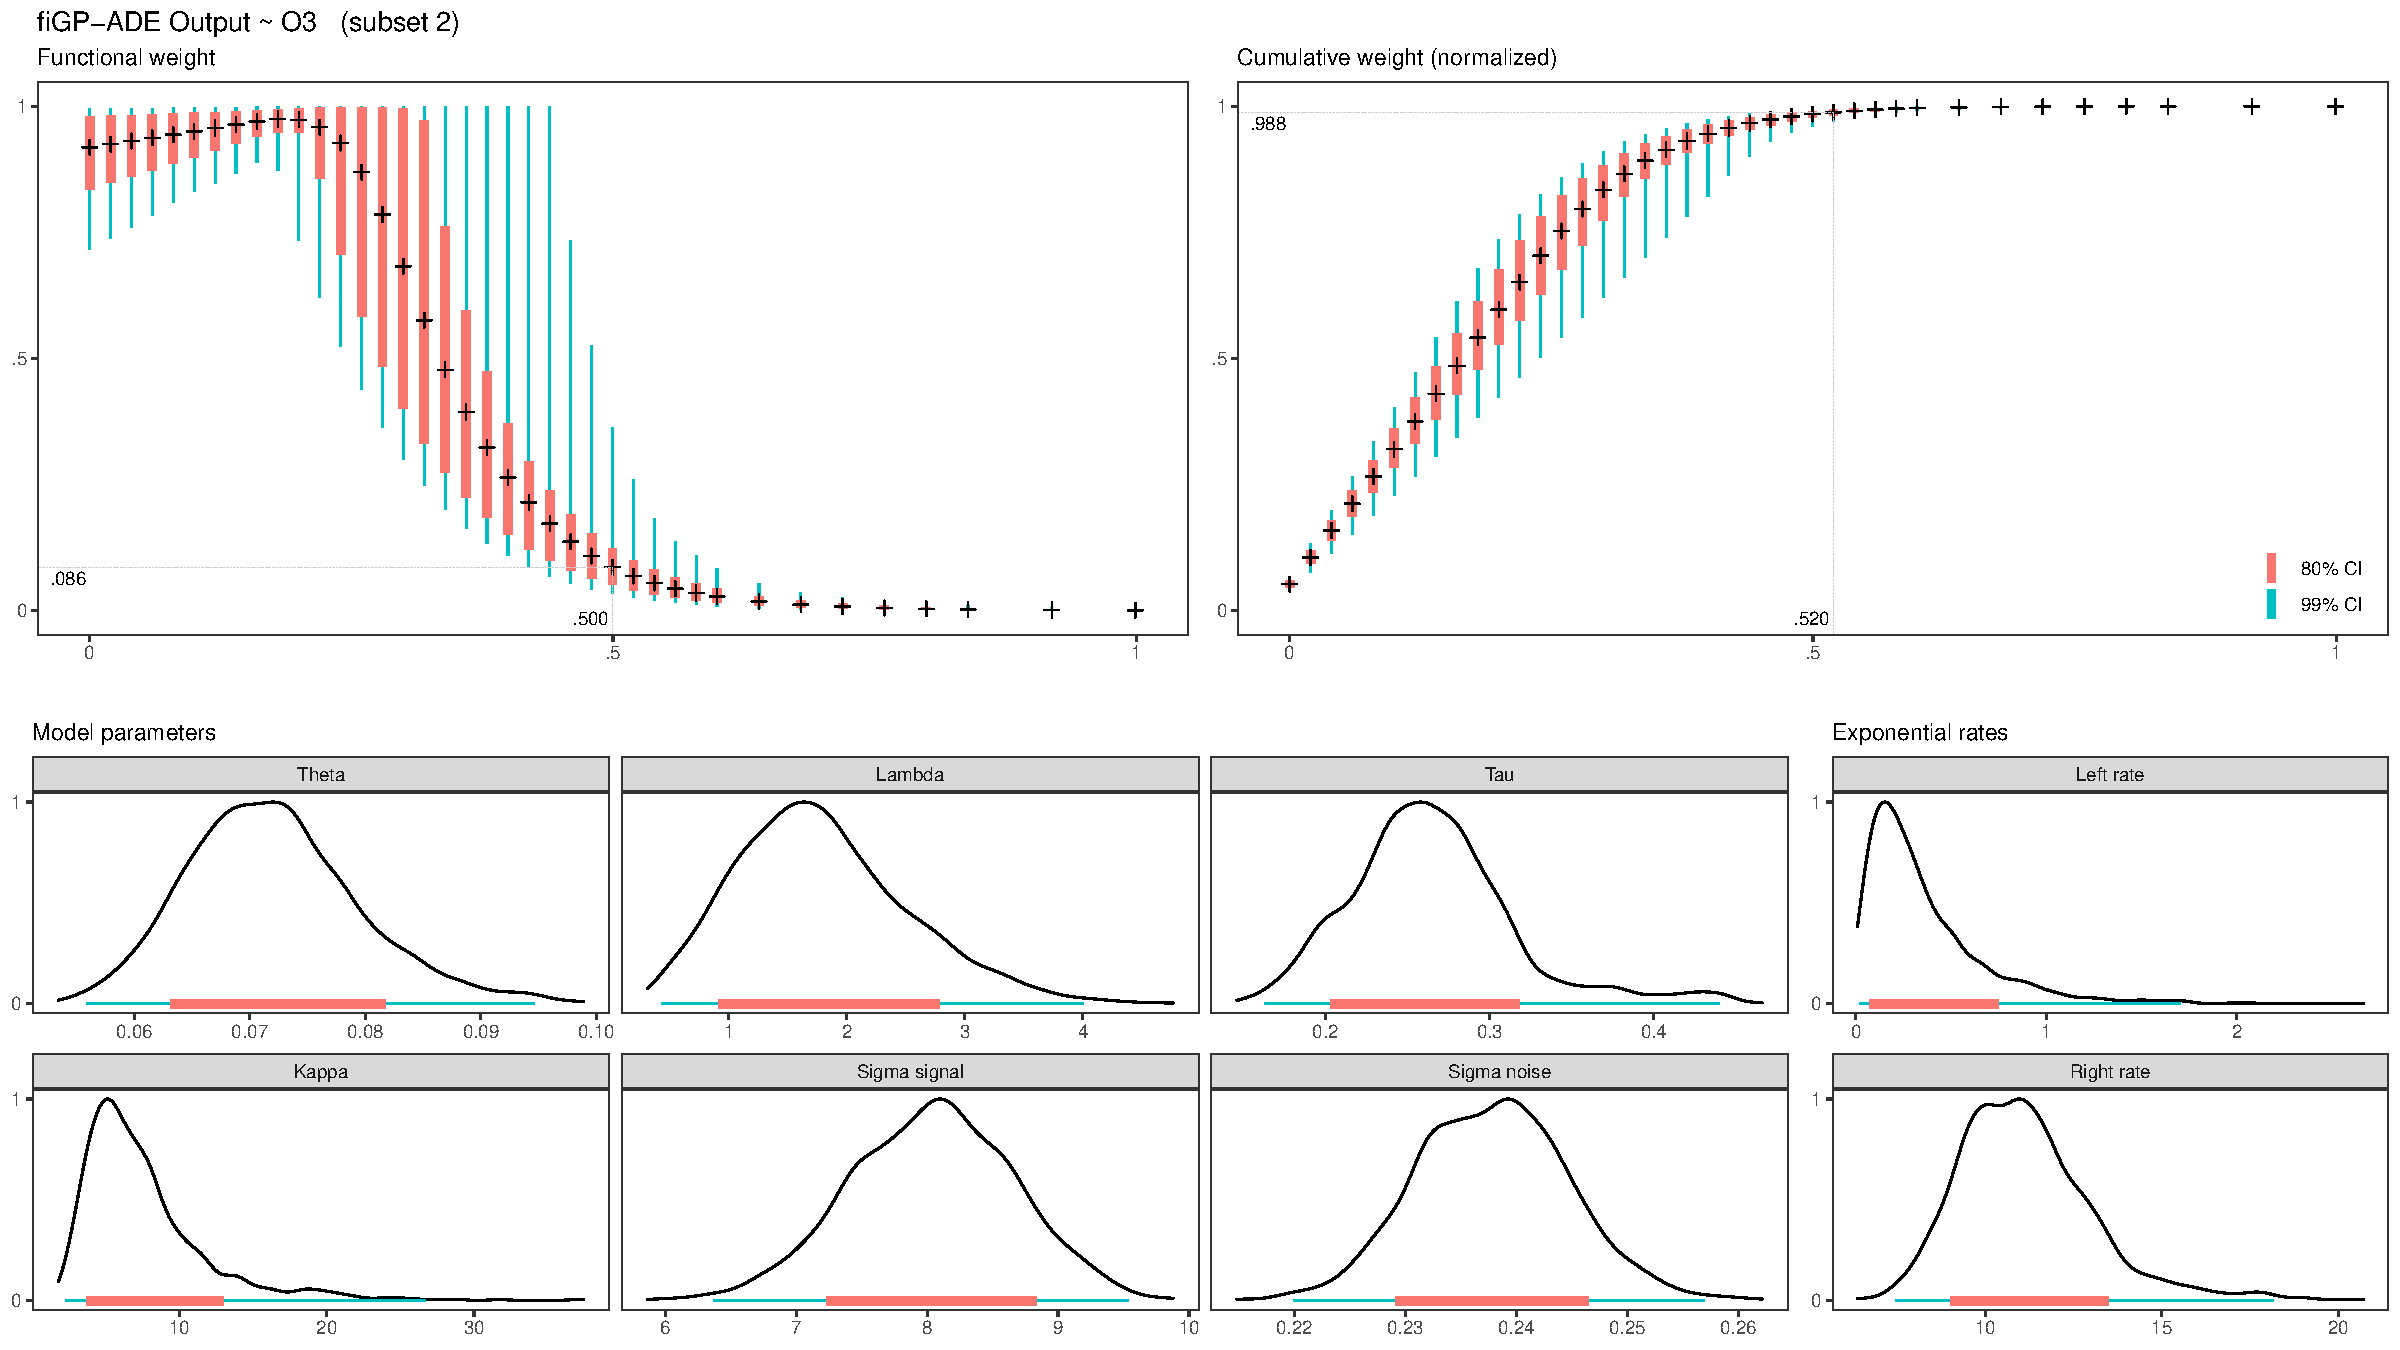
\includegraphics[width=.95\textwidth]{param-band2-unk-2-fiGP-ADE-1-O3.pdf}
  \end{figure}
\end{frame}

\begin{frame}[c]
  \begin{figure}
    \centering
    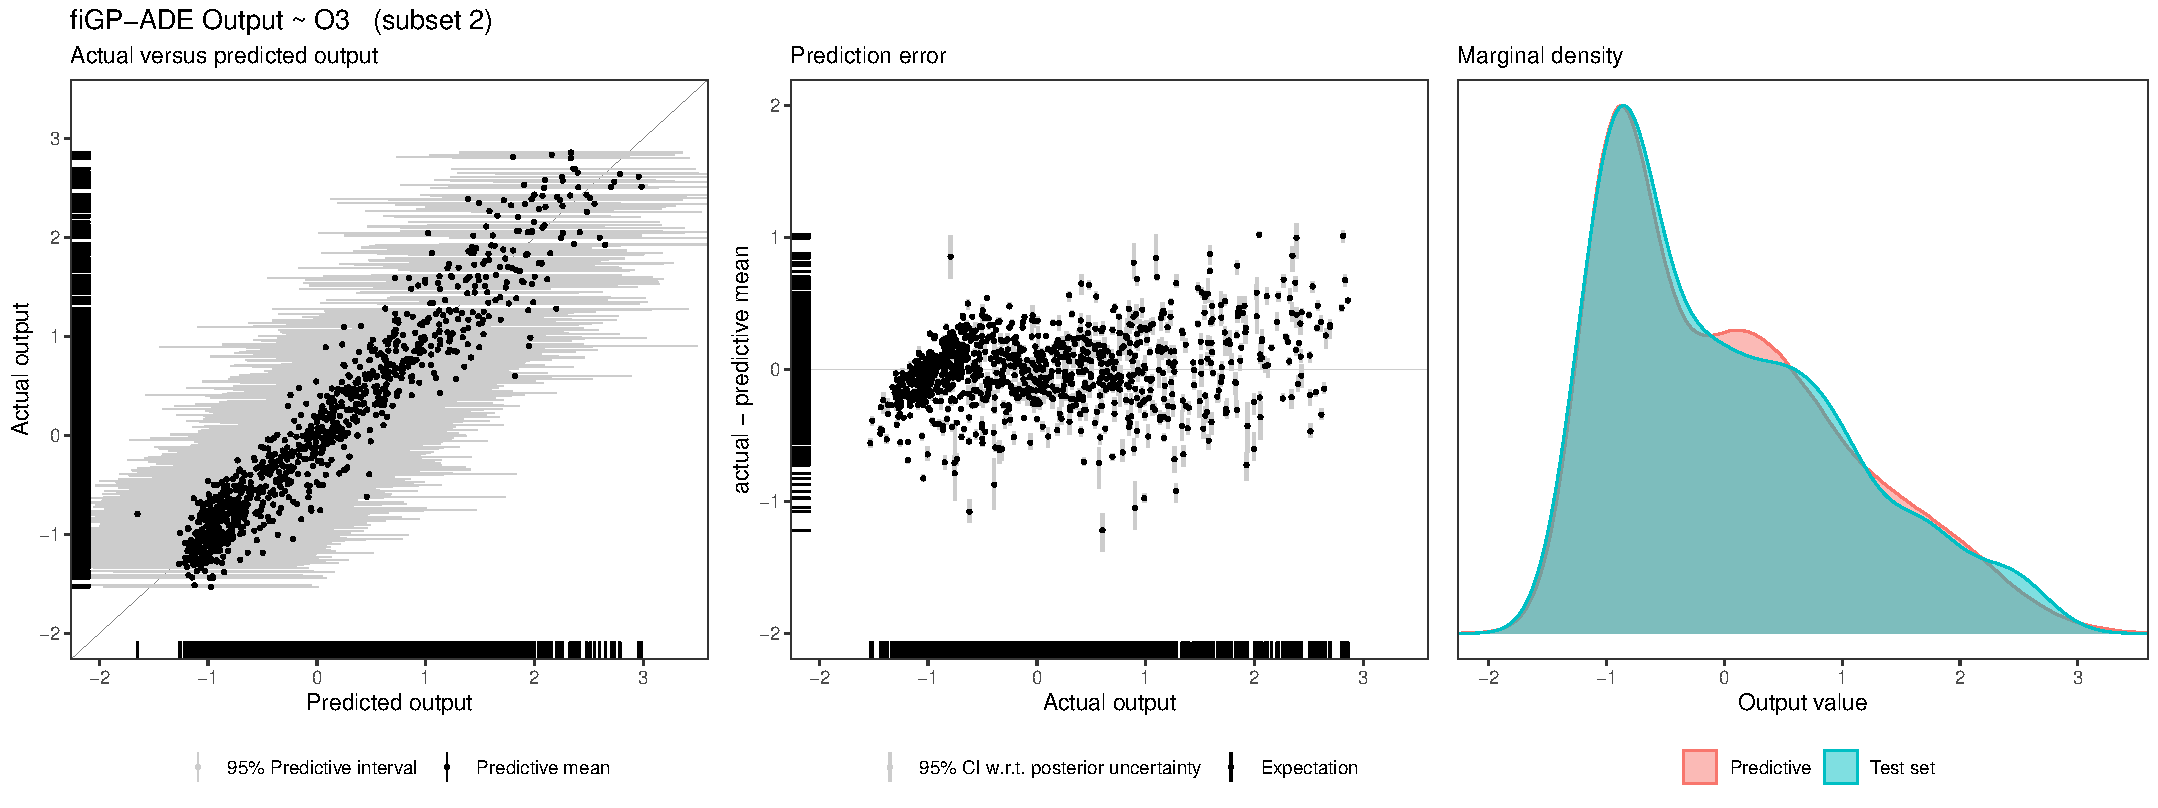
\includegraphics[width=.75\textwidth]{pred-band2-unk-2-fiGP-ADE-1-O3.pdf}
    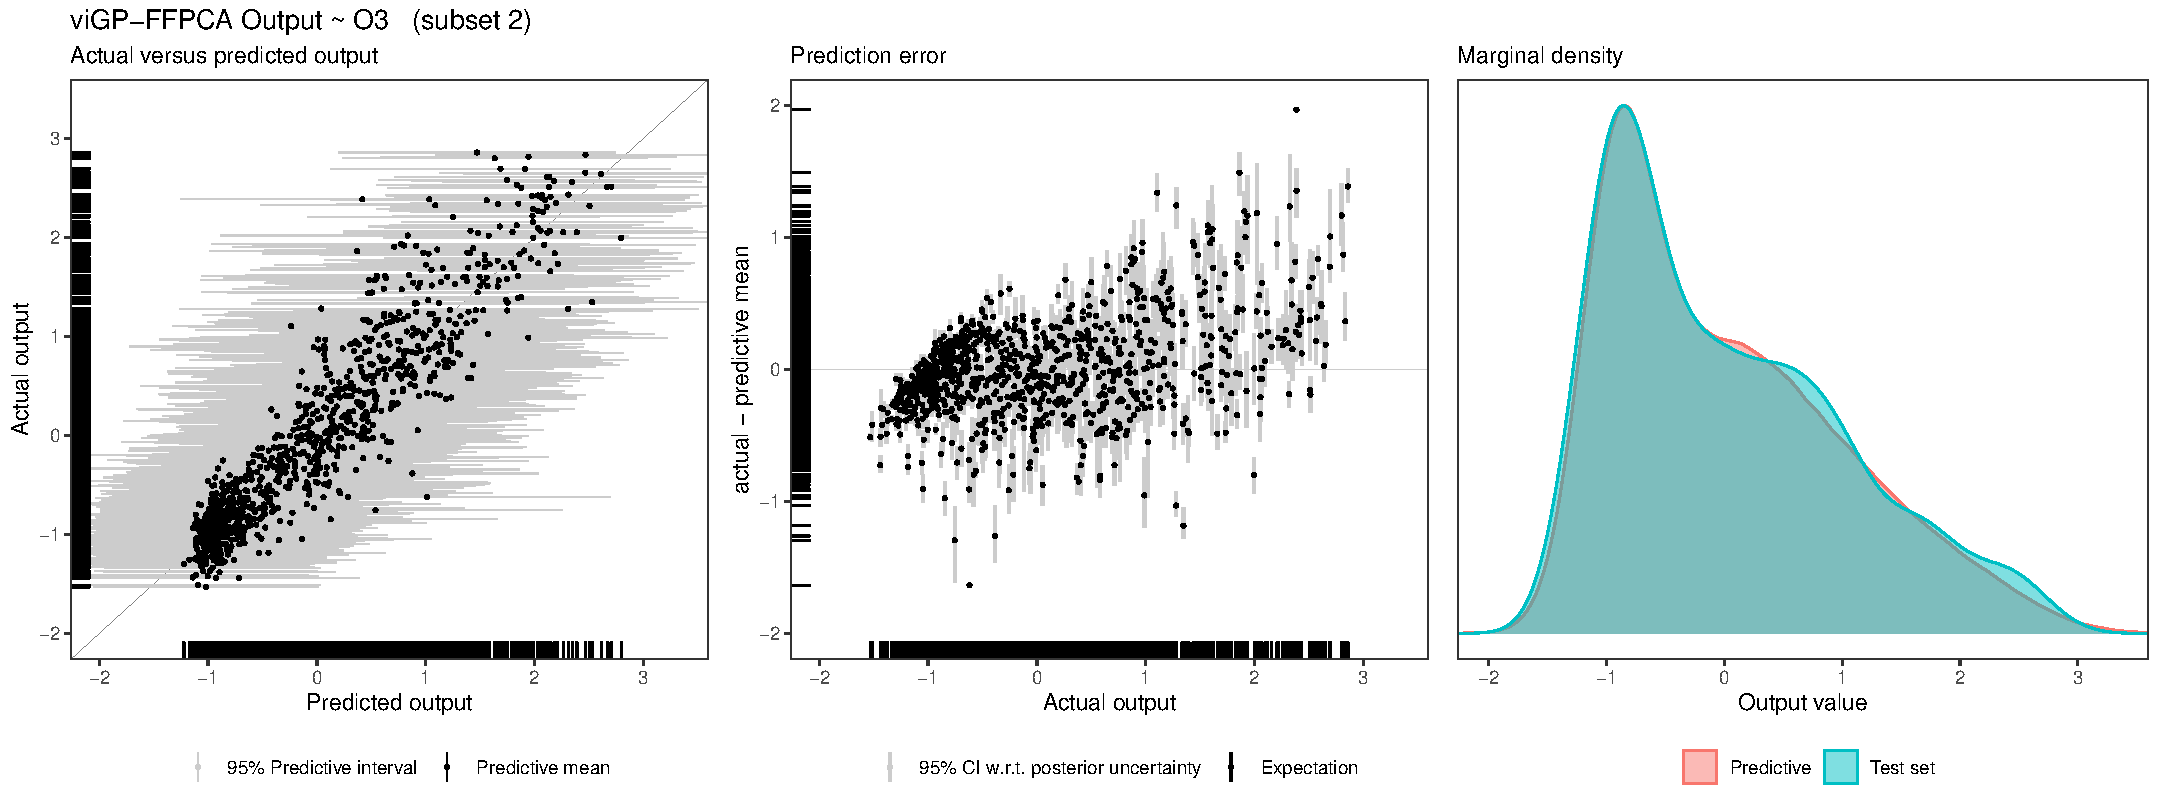
\includegraphics[width=.75\textwidth]{pred-band2-unk-2-viGP-FFPCA-1-O3.pdf}
  \end{figure}
\end{frame}

\begin{frame}%
  \label{frm:validation-statistics}
  \frametitle{Case study}
  \framesubtitle{Out-of-sample prediction}

  \begin{table}
    \adjustbox{width=0.89\textwidth}{%
      \centering
      \begin{tabular}{lrrrrr|r}
        \toprule
        % latex table generated in R 4.0.4 by xtable 1.8-4 package
% Sat Dec 11 14:39:57 2021
%  & H2O & HNO3 & N2O & O3 & Temp & Mean \\ 
%   \midrule
% \textsc{SE} &  .34 &  .48 &  .44 &  .32 &  .25 &  .37 \\ 
%   \textsc{ARD} &  .31 &  .47 &  .43 &  .30 &  .25 &  .35 \\ 
%   \textsc{FPCA} &  .67 &  .91 &  .99 &  .46 &  .54 &  .71 \\ 
%   \textsc{FFPCA} &  .46 &  .54 &  .46 &  .38 &  .33 &  .44 \\ 
%   \textsc{Edn} &  .33 &  .47 &  .44 &  .29 &  .25 &  .36 \\ 
%   \textsc{SDE} &  .31 &  .47 &  .44 &  .29 &  .25 &  .35 \\ 
%   \textsc{ADE} &  .31 &  .47 &  .43 &  .29 &  .25 &  .35 \\ 
%    \midrule
% Mean &  .39 &  .55 &  .52 &  .33 &  .31 &  .42 \\ 
%    \bottomrule
 & H2O & HNO3 & N2O & O3 & Temp & Mean \\ 
  \midrule
  \textsc{SE}    &  .34       &  {\bf .48} &  {\bf .44} &  .32       &  {\bf .25} &  .37 \\ 
  \textsc{ARD}   &  {\bf .31} &  {\bf .47} &  {\bf .43} &  {\bf .30} &  {\bf .25} &  .35 \\ 
  \textsc{FPCA}  &  .67       &  .91       &  .99       &  .46       &  .54       &  .71 \\ 
  \textsc{FFPCA} &  .46       &  .54       &  {\bf .46} &  .38       &  .33       &  .44 \\ 
  \textsc{Edn}   &  .33       &  {\bf .47} &  {\bf .44} &  {\bf .29} &  {\bf .25} &  .36 \\ 
  \textsc{SDE}   &  {\bf .31} &  {\bf .47} &  {\bf .44} &  {\bf .29} &  {\bf .25} &  .35 \\ 
  \textsc{ADE}   &  {\bf .31} &  {\bf .47} &  {\bf .43} &  {\bf .29} &  {\bf .25} &  .35 \\ 
   \midrule
   Mean          &  .39 &  .55 &  .52 &  .33 &  .31 &  .42 \\ 
   \bottomrule
      \end{tabular}
      \begin{tabular}{lrrrrr|r}
        \toprule
        % latex table generated in R 4.0.4 by xtable 1.8-4 package
% Sat Dec 11 14:39:57 2021
  %                & H2O & HNO3 & N2O & O3 & Temp & Mean \\ 
  % \midrule
  % \textsc{SE}    & 273 & 613 & 589 & 142 & -4 & 323 \\ 
  % \textsc{ARD}   & 196 & 619 & 581 & 92 & -14 & 295 \\ 
  % \textsc{FPCA}  & 1024 & 1320 & 1406 & 637 & 802 & 1038 \\ 
  % \textsc{FFPCA} & 535 & 646 & 630 & 295 & 268 & 475 \\ 
  % \textsc{Edn}   & 260 & 623 & 585 & 90 & 4 & 312 \\ 
  % \textsc{SDE}   & 202 & 623 & 585 & 85 & 4 & 300 \\ 
  % \textsc{ADE}   & 202 & 610 & 581 & 89 & 2 & 297 \\ 
  %  \midrule
  %  Mean & 385 & 722 & 708 & 204 & 152 & 434 \\ 
  %  \bottomrule
                 & H2O & HNO3 & N2O & O3 & Temp & Mean \\ 
  \midrule
  \textsc{SE}    & 273       & {\bf 614} & {\bf 585} & 138      & {\bf -7}  & 323 \\ 
  \textsc{ARD}   & {\bf 196} & {\bf 619} & {\bf 581} & {\bf 92} & {\bf -13} & 295 \\ 
  \textsc{FPCA}  & 1024      & 1320      & 1406      & 637      & 802       & 1038 \\ 
  \textsc{FFPCA} & 535       & {\bf 646} & {\bf 630} & 295      & 268       & 475 \\ 
  \textsc{Edn}   & 261       & {\bf 623} & {\bf 585} & {\bf 90} & {\bf 4}   & 312 \\ 
  \textsc{SDE}   & {\bf 202} & {\bf 623} & {\bf 585} & {\bf 85} & {\bf 4}   & 300 \\ 
  \textsc{ADE}   & {\bf 202} & {\bf 610} & {\bf 581} & {\bf 87} & {\bf 2}   & 297 \\ 
   \midrule
   Mean & 385 & 722 & 708 & 204 & 152 & 434 \\ 
   \bottomrule
      \end{tabular}}
    \caption{Mean validation statistics
      $\bar{v}^{(p, q)}$: RMSE (left) and negPPLD (right).
      Smaller values are better. Bold: best in class.}%
    \label{tab:validation-statistics-mini}
  \end{table}

  Mean validation statistics: RMSE (left) and negative posterior
  predictive log-density (right).  Smaller values are better. Bold: best
  in column. \textsc{Edn} $\tau = 0, \kappa = 1$; \textsc{SDE} $\tau =
  0$; \textsc{ADE} $\tau, \kappa, \lambda$ all free; \textsc{ARD} as
  many free parameters as measurements per vertical profile.
\end{frame}

\end{document}

%%% Local Variables:
%%% eval: (TeX-run-style-hooks "beamer")
%%% mode: latex
%%% TeX-master: t
%%% End:
